\let\cleardoublepage\clearpage
\part{Информационно-коммуникационные и химические технологии}
\chapter{Информационно-коммуникационные технологии}

{\bfseries ҒТАМР 50.41.17}
\hfill {\bfseries \href{https://doi.org/10.58805/kazutb.v.2.23-438}{https://doi.org/10.58805/kazutb.v.2.23-438}}

\sectionwithauthors{М.Қ. Жантөре, Б.С. Омаров, Г.З. Зиятбекова, Ж.Бидахмет}{МИ ИНСУЛЬТІН ДИАГНОСТИКАЛАУ ЖҮЙЕСІН КОНВОЛЮЦИЯЛЫҚ НЕЙРОНДЫҚ
ЖҮЙЕЛЕР КӨМЕГІМЕН ӘЗІРЛЕУ}

\begin{center}
{\bfseries М.Қ. Жантөре, Б.С. Омаров, Г.З. Зиятбекова\envelope, Ж.Бидахмет}

әл-Фараби атындағы Қазақ Ұлттық университеті, Алматы, Қазақстан,

е-mail: ziyatbekova@mail.ru
\end{center}

Ми инсультінің диагностикасына қатысты мәселелердің өзектілігінің артуы
аясында медициналық диагностикадағы заманауи зерттеулер осы ауыр ауруды
анықтау процесін жақсарту үшін терең оқытудың озық әдістерін қолдануға
тырысады. Бұл зерттеу инсультті анықтаудың дәлдігі мен жеделдігін
арттыру мақсатында ми инсультін диагностикалаудың қолданыстағы
әдістеріне шолу болып табылады. Деректерді өңдеуде шуды азайту, өлшемін
өзгерту және кескіндерді қалыпқа келтіру сияқты деректерді жинау, өңдеу
және күшейту әдістерін ұсынады. Нәтижелер медициналық диагностиканың
дамуына және инсультпен ауыратын науқастарға күтімнің жақсаруына
айтарлықтай ықпал етуі мүмкін. Жұмыста ми инсультін диагностикалау үшін
3D CNN қолданылды. Бұл архитектура компьютерлік томография (КТ) сияқты
үш өлшемді деректерді өңдеудің қуатты құралы болып табылады. Модельдің
өнімділігін бағалау дәлдік, шолу және F1-бағалау сияқты әртүрлі
көрсеткіштерді пайдалануды қамтиды. 3D CNN ми инсультін диагностикалауда
жоғары көрсеткіштерге қол жеткізді, соның ішінде аралық күшейтуді
қолданғанда 0.9310 дәлдікті және 0.8636 еске түсіру коэффицентін
көрсетті.

{\bfseries Түйін сөздер}: Ми инсульті, анықтау, 3D CNN, кушейту,
аугментация.

\begin{center}
{\large\bfseries РАЗРАБОТКА СИСТЕМЫ ДИАГНОСТИКИ ИНСУЛЬТА ГОЛОВНОГО МОЗГА С
ПОМОЩЬЮ СВЕРТОЧНЫХ НЕЙРОННЫХ СИСТЕМ}

{\bfseries М.К. Жанторе, Б.С. Омаров, Г.З. Зиятбекова\envelope, Ж.Бидахмет}

Казахский национальный университет имени аль-Фараби, Алматы, Казахстан

е-mail: ziyatbekova@mail.ru
\end{center}

На фоне растущей актуальности вопросов, связанных с диагностикой
инсульта головного мозга, современные исследования в области медицинской
диагностики пытаются использовать передовые методы глубокого обучения
для улучшения процесса выявления этого серьезного заболевания.

Это исследование представляет собой обзор существующих методов
диагностики инсульта головного мозга с целью повышения точности и
оперативности обнаружения инсульта. Предоставляет методы сбора,
обработки и усиления данных, такие как шумоподавление, изменение размера
и нормализация изображений при обработке данных. Результаты могут
значительно способствовать развитию медицинской диагностики и улучшению
ухода за пациентами, перенесшими инсульт.

В работе использовался 3D CNN для диагностики инсульта головного мозга.
Эта архитектура является мощным инструментом для обработки трехмерных
данных, таких как компьютерная томография (КТ).

Оценка производительности модели включает использование различных
показателей, таких как точность, обзор и оценка F1. 3D CNN добился
высоких показателей в диагностике инсульта головного мозга, в том числе
показал точность 0,9310 и коэффициент отзыва 0,8636 при использовании
промежуточного усиления.

{\bfseries Ключевые слова:} мозговой инсульт, обнаружение, 3D CNN,
усиление, аугментация.
\newpage
\begin{center}
{\large\bfseries DEVELOPMENT OF A BRAIN STROKE DIAGNOSIS SYSTEM USING
CONVOLUTIONAL NEURAL SYSTEMS}

{\bfseries M.K. Zhantore, B.S. Omarov, G.Z. Ziyatbekova\envelope, Zh.Bidakhmet}

Al-Farabi Kazakh National University, Almaty, Kazakhstan,

е-mail:ziyatbekova@mail.ru
\end{center}

Against the background of the growing relevance of issues related to the
diagnosis of brain stroke, modern research in the field of medical
diagnostics is trying to use advanced deep learning methods to improve
the detection of this serious disease.

This study provides an overview of existing methods for diagnosing brain
stroke in order to improve the accuracy and efficiency of stroke
detection. Provides methods for collecting, processing, and amplifying
data, such as noise reduction, resizing, and normalization of images
during data processing. The results can significantly contribute to the
development of medical diagnostics and improve the care of stroke
patients.

The work used 3D CNN to diagnose a brain stroke. This architecture is a
powerful tool for processing three-dimensional data such as computed
tomography (CT).

Model performance evaluation includes the use of various indicators such
as accuracy, review and F1 score. 3D CNN has achieved high rates in the
diagnosis of cerebral stroke, including showing accuracy of 0.9310 and a
recall coefficient of 0.8636 when using intermediate gain.

{\bfseries Keywords:} brain stroke, detection, 3D CNN, cushioning,
augmentation.

\begin{multicols}{2}
{\bfseries Кіріспе.} Қазіргі уақытта ми инсультін диагностикалауға
байланысты проблемалар медициналық диагностика мен емдеу саласында
өзекті бола түсуде {[}1{]}. Орталық жүйке жүйесінің ең ауыр ауруларының
бірі ретінде ми инсульті мүмкіндігінше тиімді емдеу және ықтимал
асқынулардың алдын алу үшін жедел және дәл диагностиканы қажет етеді
{[}2{]}.

Осыған байланысты медициналық диагностика саласындағы заманауи
зерттеулер ми инсультін диагностикалаудың күрделі мәселелерін шешудің
перспективалық тәсілдерін ұсына отырып, терең оқыту технологияларын
белсенді түрде енгізуде. Мұндай инновациялық әдістерді қолдану
медициналық суреттердегі инсульт белгілерін анықтаудың дәлдігі мен
жеделдігін едәуір жақсарта алады, диагноз қою мен емдеуді бастау
арасындағы уақытты қысқартады {[}3{]}.

Осы тұрғыда бұл мақала терең оқытуды қолдана отырып, ми инсультін
диагностикалау жүйесін зерттеуге және дамытуға бағытталған. Біз
қолданыстағы диагностикалық әдістерге және олардың шектеулеріне шолу
жасаймыз және ми инсультінің диагностикалық процесін жақсартуға арналған
3D конволюциялық нейрондық желі архитектурасын ұсынамыз. Сонымен қатар,
мақалада шуды жою, өлшемін өзгерту және кескіндерді қалыпқа келтіру
сияқты медициналық деректерді өңдеу мен дайындаудың маңызды аспектілері
қамтылған. Деректерді өңдеудің осы кезеңдерін талдау модельді оқыту үшін
кірістердің жоғары сапасын қамтамасыз ету үшін өте маңызды {[}4{]},
сондықтан оның жалпылау қабілетін арттырады.

Тұтастай алғанда, бұл жұмыс Медициналық диагностика саласын дамытуға
және инсультпен ауыратын науқастарға күтімді жақсартуға маңызды үлес
бола алатын терең оқытуды пайдалана отырып, ми инсультін
диагностикалауға жан-жақты шолу мен заманауи көзқарасты қамтамасыз ету
міндетін қояды.

Соңғы онжылдықта терең оқыту, әсіресе конволюциялық нейрондық желілер
(CNN) медициналық диагностика саласында қуатты құралға айналды {[}5{]}.
Бұл технологиялар медициналық суреттерден күрделі үлгілерді автоматты
түрде алу қабілетін көрсетеді, бұл оларды инсульт диагностикасының
перспективалы құралы етеді {[}6{]}.

Бұл мақалада біз мидың компьютерлік томографиясына (CT) негізделген
терең оқытуды қолдана отырып, ми инсультін диагностикалау әдісін
қарастырамыз. 3D конволюциялық нейрондық желілерді қолдану, сондай-ақ
деректер мен оқу процесін оңтайландыру осы ауыр неврологиялық аурумен
күресуде жаңа көкжиектерді ашу арқылы диагностиканың дәлдігі мен
жеделдігін жақсартуға мүмкіндік береді {[}7{]}.

{\bfseries Материалдар мен әдістер.} Соңғы онжылдықтарда ми инсультін
диагностикалау саласында әсерлі өсу байқалды, бұл осы саладағы әдістер
мен технологияларды жетілдіруге бағытталған көптеген зерттеулердің пайда
болуымен байланысты {[}8{]}. Терең оқыту технологияларының дамуы
диагностиканың дәлдігі мен жеделдігін жақсартудың жаңа перспективаларын
ұсына отырып, осы процеске белсенді әсер етеді.

Бұрын жүргізілген зерттеулер ми инсультінің медициналық диагностикасында
қолданылатын әдістерге Негізгі шолу жасайды. Компьютерлік томография
(КТ) және магнитті-резонанстық томография (МРТ) сияқты дәстүрлі әдістер
ұзақ уақыт бойы ми құрылымындағы өзгерістерді анықтаудың негізгі құралы
болды. Дегенмен, олардың кең қолданылуына қарамастан, олардың
сезімталдығы мен ерекшелігінде шектеулер бар, бұл тиімдірек әдістерді
табу қажеттілігін көрсетеді {[}9{]}.

Анықтамалық векторлық әдіс (SVM) және кездейсоқ ормандар сияқты
Машиналық оқыту әдістерінің пайда болуы диагностиканы жақсартудағы
маңызды қадам болды {[}10{]}. Бұл тәсілдер медициналық кескіндерді
талдау процесін автоматтандыруға мүмкіндік береді, бірақ көбінесе
күрделі үш өлшемді деректер мен үлкен көлемдегі ақпаратты өңдеуде
шектеулерге тап болады.

Терең оқыту саласындағы соңғы зерттеулер ми инсультін диагностикалау
мәселелерін шешудің перспективалық тәсілдерін ұсынады. Нейрондық
желілердің архитектуралары, соның ішінде конволюциялық нейрондық желілер
(CNN) және қайталанатын нейрондық желілер (RNN) деректердегі кеңістіктік
және уақыттық тәуелділіктерді ескере отырып, жоғары дәлдікті қамтамасыз
етеді {[}11{]}.

Медициналық тәжірибелерде ақпараттық технологиялардың пайда болуымен
диагностиканың әртүрлі модельдерін медициналық ақпараттық жүйелерге
біріктіру үрдісі байқалады {[}12{]}. Зерттеудің бұл бағыты диагностика
процесін оңтайландыруға, сондай-ақ медициналық ақпараттың қолжетімділігі
мен алмасуын арттыруға бағытталған.

Ми инсультінің диагностикасын зерттеу үшін Kaggle платформасынан
жиналған мәліметтер жиынтығы қолданылды (1-сурет). Суреттердің жалпы
саны 2501 құрайды, оның ішінде қалыпты жағдайы бар 1551 сурет және
инсульт белгілері бар 950 сурет.
\end{multicols}

\begin{figure}[H]
	\centering
	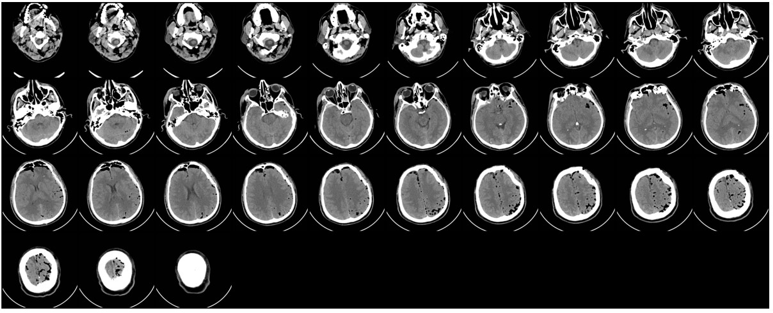
\includegraphics[width=0.7\textwidth]{assets/1}
	\caption*{1-сурет -- Пациенттің суреттер жиынтығы}
\end{figure}

\begin{multicols}{2}
Деректердегі әрбір суретте "patient\_id (SLICE\_ID)" форматында бірегей
атау бар.jpg", мұнда patient\_id пациенттің идентификаторын, ал
SLICE\_ID - кесілген Нөмірді білдіреді. Бұл деректерді жүйелеуге және
оларды белгілі бір пациенттермен және уақыт нүктелерімен байланыстыруға
мүмкіндік береді.

Модельдеуді бастамас бұрын, деректерді мұқият өңдеу керек. Бұл процесс
бірнеше маңызды қадамдарды қамтиды.

Шуды жою: суреттердің сапасын жақсарту үшін шуды өңдеу жүргізілді.
Кеңейту, артефактілерді жою және бинаризация сияқты морфология әдістерін
қолдана отырып, кескіндердің тазалығына қол жеткізілді. Өлшемді өзгерту:
біркелкі болу және есептеу күрделілігін азайту үшін кескіндер біркелкі
өлшемге өзгертілді. Бұл қадам кескіндерді айналдыруды, бикубикалық
интерполяция әдісін қолдана отырып олардың өлшемдерін өзгертуді және
қайта айналдыруды қамтиды. Қалыпқа келтіру: қалыпқа келтіру пиксель
мәндерін {[}0, 1{]} аралығына келтірудің маңызды кезеңі болып табылады.
Бұл деректерді стандарттауды қамтамасыз етеді және модельдік оқытуды
жақсартады {[}13{]}.

Деректерді түзету процесінде сөздік жасалды, онда әр пациент суреттердің
дұрыс сұрыпталған тізіміне сәйкес келеді. Бұл сөздік кейінгі талдау мен
модель құрудың маңызды құралына айналды.
\end{multicols}

\begin{figure}[H]
	\centering
	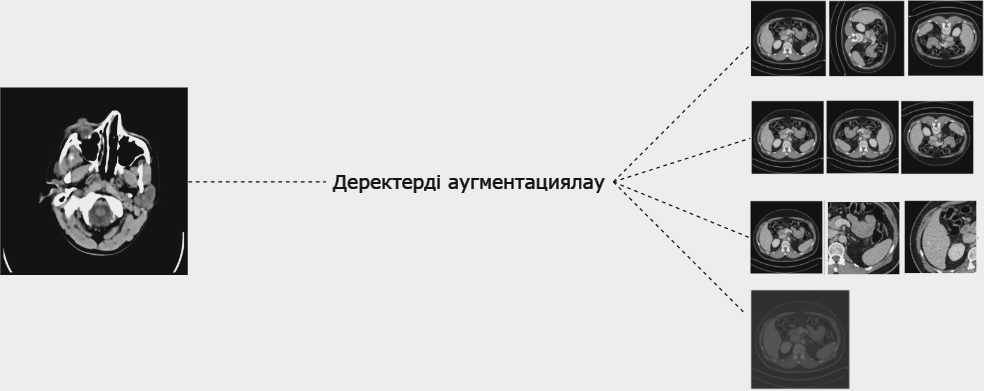
\includegraphics[width=0.7\textwidth]{assets/2}
	\caption*{2-сурет -- Күшейтудің қолданылуы}
\end{figure}

\begin{multicols}{2}
Модельді оқыту үшін деректерді дайындау процесінде әдістерді қамтитын
күшейту әдісі қолданылды (2-сурет): айналу (айналу), шағылысу (флип),
ауысу (shift), масштабтау (zoom), жылжыту (shear), жарықтықты өзгерту
(brightness) және контраст (контраст). Бұл күшейту әдістері модельдің
жалпылау қабілетін жақсартуда және оның деректердің әртүрлі
вариацияларына төзімділігін арттыруда шешуші рөл атқарады {[}14{]}.

Айналу, шағылысу, жылжыту және масштабтау сияқты деректерді күшейту
әдістері оқу жинағын әртүрлі кескін вариацияларымен байытады {[}15{]},
бұл модельге әртүрлі нысан позициялары мен масштабтарында жақсырақ
үйренуге көмектеседі. Бұл модельдің нақты көріністердегі объектілерді
тану және жіктеу қабілетін жақсартуға ықпал етеді.

Сонымен қатар, жарықтық пен контрастты өзгерту әдістері әртүрлі
жарықтандырумен және контрастпен кескіндер жасауға мүмкіндік береді, бұл
сонымен қатар, модельге әртүрлі жарық жағдайларында үйренуге
көмектеседі. Бұл модельдің жарықтандырудың өзгеруіне төзімділігін
арттырады және нақты жұмыс жағдайында тұрақты нәтижелерді қамтамасыз
етеді.

Тұтастай алғанда, осы әдістерді қолдана отырып, деректерді күшейтуді
қолдану әртүрлі және репрезентативті оқыту деректер жиынтығын құруға
ықпал етеді, бұл өз кезегінде модельдің жалпылау қабілетін жақсартады
және нақты жағдайларда деректердің әртүрлі вариацияларымен жұмыс істеу
кезінде оның тиімділігін арттырады.

Ми инсультін диагностикалау саласында терең оқыту модельдерінің озық
архитектуралары кеңінен қолданылады {[}16{]}. Бұл шолуда біз негізгі
архитектураны қарастырамыз - көлемдегі медициналық кескіндерді талдауға
арналған 3D конволюциялық нейрондық желі (3D CNN). Бұл желі белгілерді
анықтауда керемет тиімділікті көрсетеді және ми инсультін дәл
диагностикалауға мүмкіндік береді.

3D CNN-медициналық суреттер сияқты үш өлшемді деректермен жұмыс істеуге
арнайы бейімделген классикалық конволюциялық нейрондық желі
архитектурасының дамуы. Ол үш өлшемді кеңістіктегі кеңістіктік және
уақыттық белгілерді бөлектеу үшін үш өлшемді конволюцияларды пайдалану
идеясына негізделген. 3D cnn негізгі ерекшеліктері:

\begin{enumerate}
\def\labelenumi{\arabic{enumi}.}
\item
  Үш өлшемді конволюциялар: 3D CNN көлемді деректерді талдау үшін үш
  өлшемді конволюцияларды пайдаланады. Бұл уақыт осі бойындағы
  кеңістіктік тәуелділіктер мен белгілердің өзгеруін ескеруге мүмкіндік
  береді.
\item
  Пулинг: конволюцияларға ұқсас, көлемді пиллинг операциялары есептеу
  көлемін азайтуға және негізгі белгілерді алуға көмектесетін
  деректердің өлшемін азайту үшін қолданылады.
\item
  Адаптивті архитектура: 3D CNN кіріс деректерінің өлшемдері мен
  пішімдерінің өзгеруіне оңай бейімделеді, бұл оны әртүрлі өлшемдегі
  медициналық кескіндерді талдаудың қуатты құралына айналдырады.
\end{enumerate}

Ми инсультін диагностикалауда қолдану:

\begin{enumerate}
\def\labelenumi{\arabic{enumi}.}
\item
  Ерекшеліктерді бөлектеу: 3D CNN медициналық суреттерде қанайналым
  жүйесіндегі ауытқулар немесе ми құрылымындағы өзгерістер сияқты
  сипаттамалық ерекшеліктерді ажырата алады.
\item
  Дені сау және зардап шеккен аймақтарды саралау: Архитектура инсультті
  диагностикалау үшін маңызды болып табылатын мидың қалыпты және зардап
  шеккен аймақтары арасында дәл ажыратуға мүмкіндік береді.
\item
  Кеңістіктік және уақыттық тәуелділіктерді есепке алу: 3D CNN
  деректердегі үш өлшемді кеңістіктік және уақыттық тәуелділіктерді
  тиімді қарастырады, бұл диагностиканың дәлдігін жақсартады және тіпті
  күрделі өзгерістерді анықтауға мүмкіндік береді {[}17{]}.
\end{enumerate}

Бұл жұмыста ми инсультін диагностикалау үшін 3D конволюциялық нейрондық
желі қолданылды. Бұл архитектура компьютерлік томография (CT) сияқты үш
өлшемді деректерді өңдеуге арналған қуатты құрал болып табылады
(3-сурет).
\end{multicols}

\begin{figure}[H]
	\centering
	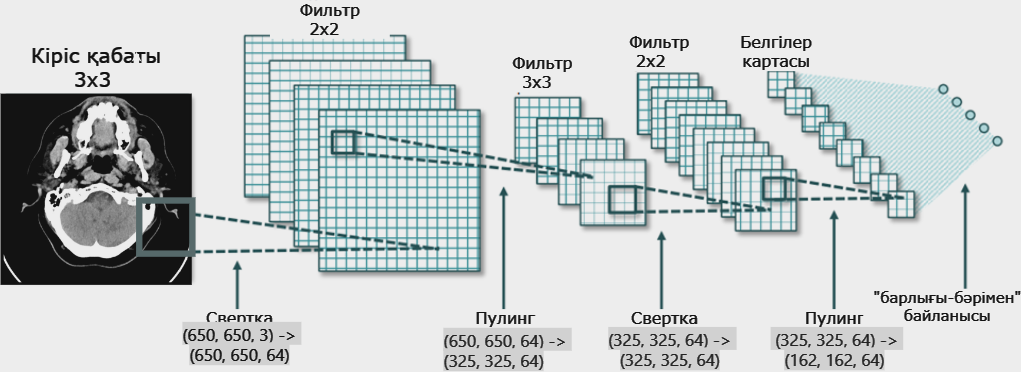
\includegraphics[width=0.7\textwidth]{assets/3}
	\caption*{3-сурет -- 3D CNN архитектурасы}
\end{figure}

\begin{multicols}{2}
Бұл бөлімде ми инсультін диагностикалау үшін ұсынылған модельдің
архитектурасы қарастырылады. Негізгі құрал 3D конволюциялық нейрондық
желі болып табылады, ол үш өлшемді кірістерді тиімді өңдеуді қамтамасыз
етеді.

3D конволюциялық нейрондық желінің жұмыс принципі оның үш өлшемді
деректерді талдау қабілетінде жатыр, бұл әсіресе CT сканерлері сияқты
медициналық кескіндерді өңдеу кезінде маңызды. Бұл архитектура көлемді
деректердегі кеңістіктік ерекшеліктер мен қатынастарды алуға мүмкіндік
береді.

Модель архитектурасы бірнеше негізгі қабаттарды қамтиды, олардың
әрқайсысы деректерді өңдеу мен талдауда шешуші рөл атқарады. Кіріс
қабаты үш өлшемді CT сканерлеуді қабылдауға арналған, ал конволюция
қабаттары үш өлшемді кеңістіктен белгілерді шығарып, үш бағытта
(тереңдік, ені, биіктігі) конволюция операцияларын орындайды.

Сонымен қатар, модельге деректердің көлемін азайту және негізгі
белгілерді сақтау арқылы олардың өлшемін төмендететін Max Pooling
қабаттары сияқты кіші үлгі қабаттары кіреді. Бұл компоненттер үш өлшемді
медициналық кескіндерге негізделген тиімді оқыту мен диагностика үшін
оңтайлы архитектураны қамтамасыз етеді {[}18{]}.

Терең оқытуды қолдана отырып, ми инсультін диагностикалау жүйесін
дамытудағы маңызды қадам модельдің өнімділігін бағалау болып табылады.
Ол үшін жүйенің дәлдігін, сезімталдығын және басқа сипаттамаларын
өлшеуге мүмкіндік беретін әртүрлі көрсеткіштер мен көрсеткіштер
қолданылады. Төменде әзірленген модельдің тиімділігін бағалау үшін
қолданылатын негізгі бағалау көрсеткіштеріне шолу берілген.

Дәлдік мысалдардың жалпы санына қатысты модельдің дұрыс болжамдарының
пайызын білдіреді {[}19{]}. Бұл көрсеткіш жүйенің тиімділігінің жалпы
өлшемі болып табылады және формула бойынша есептеледі:

Дәлдік = Дұрыс болжамдардың саны/Мысалдардың жалпы саны

Шолу (немесе сезімталдық) модельдің оң жағдайларды анықтау қабілетін
өлшейді. Бұл ми инсультін диагностикалау контекстіндегі маңызды
көрсеткіш, өйткені жалған теріс нәтижелердің төмендеуі өте маңызды
{[}20{]}. Шолу формула бойынша есептеледі:

Шолу = Шынайы оң болжамдардың саны/Нақты оң жағдайлардың жалпы саны

F1-бағалау дәлдік пен шолудың орташа өлшенген мәні болып табылады. Бұл
көрсеткіш жалған оң және жалған теріс жағдайларды ескереді, бұл
теңгерімсіз деректермен жұмыс істеу кезінде оны ақпараттандырады
{[}21{]}.

\hspace{0pt} {\bfseries Нәтижелер мен талқылау.} Зерттеу барысында әртүрлі
оқу параметрлерінің конфигурацияларын қолдана отырып, модель әзірленді
және оқытылды. Оқыту дәуірлерінің жалпы саны 150 болды және олардың
әрқайсысы үшін модель төрт түрлі жағдайда сыналды, соның ішінде
деректерді күшейтудің әртүрлі комбинациялары ұсынылды (1-кесте).

Күшейтудің болмауы: бұл режимде барлық күшейту қабаттары өшірілді, бұл
модельге бастапқы деректерде өзгеріссіз үйренуге мүмкіндік берді.

Негізгі күшейту: бұл режим тек жарықтық пен контрастты өзгерту
қабаттарын қамтыды. Күшейтудің бұл түрі модельге кескіндердің жарықтығы
мен контрастының өзгеруіне төзімді болуға көмектесті.

Аралық күшейту: жарықтықты, контрастты, бұрылысты, шағылысуды және орын
ауыстыруды өзгерту қабаттарын қамтыды. Ұлғайтудың бұл түрі оқу деректер
жиынтығының әртүрлілігіне ықпал етті және модельдің кірістердің әртүрлі
вариацияларына төзімділігін арттырды.

Жетілдірілген күшейту: барлық қол жетімді күшейту қабаттарын қамтыды.
Күшейтудің бұл түрі жарықтылықтың, Контрасттың, бұрылыстардың,
шағылысулардың, мещысулардың және басқа кескін түрлендірулерінің
өзгеруін қоса алғанда, оқу деректер жиынтығында максималды әртүрлілікті
қамтамасыз етті.
\end{multicols}

\begin{table}[]
\caption*{1-кесте -- Күшейту түрі бойынша бағалау}
\centering
\begin{tabular}{|l|l|l|}
\hline
Күшейту түрі & Дәлдік & Шолу \\ \hline
Күшейтудің болмауы & 0.9655 & 0.9091 \\ \hline
Негізгі күшейту & 0.9828 & 0.9545 \\ \hline
Аралық күшейту & 0.9310 & 0.8636 \\ \hline
Кеңейтілген күшейту & 0.8793 & 0.8182 \\ \hline
\end{tabular}%
\end{table}

\begin{figure}[H]
	\centering
	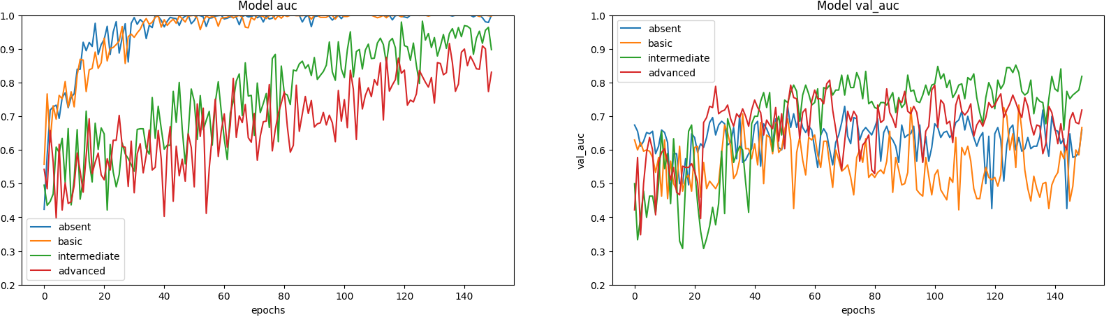
\includegraphics[width=0.9\textwidth]{assets/4}
	\caption*{(a)}
\end{figure}

\begin{figure}[H]
	\centering
	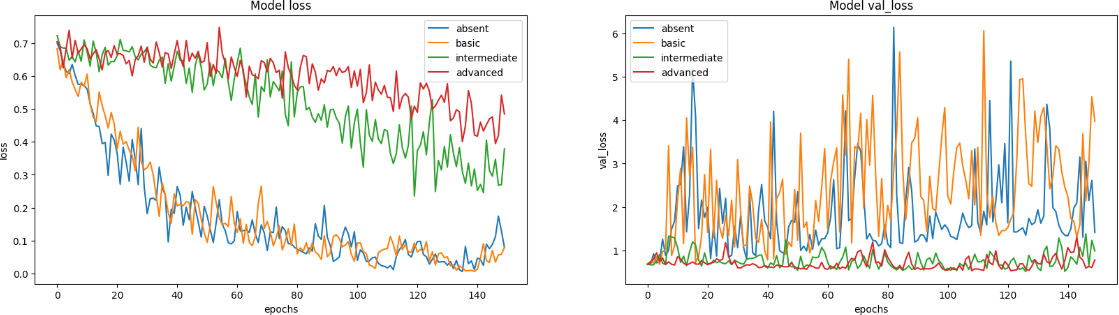
\includegraphics[width=0.9\textwidth]{assets/5}
	\caption*{(b)}
	\caption*{4-сурет -- 150 эпохадағы модельді сынау (a) дәлдік (b) тестілеу және валидация кезіндегі шығын}
\end{figure}

\begin{multicols}{2}
4-суретте модельдің 150 кезеңнен (эпохадан) өткеннен кейінгі тестілеу
нәтижесі диаграмма түрінде көрсетілген. Осыған қарай отырып, біздің
модельдің әр түрлі күшейту түріне байланысты дәлдіктің әртүрлі болатынын
көруге болады. Күшейтудің барлық түрін қолданғанда деректердің көлемі
үлкейіп, оның дәлдікке әсер еткенін көрсетеді. Күшейтуді қоспағанда
дәлдік 97\% және қосқанда 88\% көбейгенін көреміз.

Оқу процесі аяқталғаннан кейін модельдің тиімділігінің ақпараттық
көрінісін жасауға болады. Валидациялық деректер жиынтығындағы
теңгерімсіздікті ескере отырып, жоғарыда айтылғандай, ROC (ROC AUC)
қисығының астындағы аймақ қолданылады. Бұл метрикалық көрсеткіш
модельдің сезімталдықты да, ерекшелікті де ескере отырып, әртүрлі
сыныптар арасындағы айырмашылықты анықтау қабілетін жан-жақты бағалауды
қамтамасыз етеді. ROC AUC модельдің кемсітушілік қабілетіне нюансты баға
береді, әсіресе сыныпты бөлуде теңгерімсіздік бар сценарийлерде құнды.

Зерттеу нәтижелері ми инсультін диагностикалау үшін әзірленген модельдің
өнімділігіне әртүрлі деректерді күшейту әдістерінің айтарлықтай әсерін
көрсетеді. Эксперименттер күшейтудің төрт түрін талдады: күшейтудің
болмауы, негізгі күшейту, аралық күшейту және кеңейтілген күшейту.

Деректерді күшейтуді қолданбай оқытылған Модель жоғары дәлдікті
(96.55\%) және шолуды (90.91\%) көрсетті. Алайда, күшейтудің әртүрлі
түрлерін қосу нәтижелердің одан әрі жақсаруына әкелді. Мысалы, негізгі
күшейтуді қолдана отырып дайындалған модель дәлдікті (98.28\%) және
шолуды (95.45\%) көрсетті. Бұл суреттердің жарықтығы мен контрастын
өзгерткен кезде модельдің деректерді дұрыс жіктеу қабілетінің
айтарлықтай жақсарғанын көрсетеді.

Айта кету керек, айналу, шағылысу және орын ауыстыру сияқты қосымша
кескін түрлендірулерін қамтитын аралық және кеңейтілген күшейтуді
қолдану модельдің өнімділігін жақсартуға әкелді. Алайда, жетілдірілген
күшейтуді қолдану кезінде басқа күшейту түрлерімен салыстырғанда
дәлдіктің (87.93\%) және шолудың (81.82\%) шамалы төмендеуі байқалды.

4-суреттегі нәтижелерді талдау 150 оқу дәуіріндегі модельдің өнімділігін
нақты салыстыруға мүмкіндік береді. Дәлдік графиктері мен жоғалту
функциялары әр түрлі күшейту әдістерін қолдану түпкілікті нәтижеге
айтарлықтай әсер ететіндігін көрсетеді. Бұл терең оқыту модельдерін
оқыту үшін деректерді күшейту стратегиясын дұрыс таңдаудың маңыздылығын
растайды.

Сонымен қатар, бұл зерттеу модельдің сезімталдық пен ерекшелікті ескере
отырып, сыныптарды ажырату қабілетін бағалау үшін ROC қисығының
астындағы аймақ метрикасын (ROC AUC) пайдаланды. Нәтижелер модельдің
жоғары кемсітушілік қабілетін көрсетеді, әсіресе сынып теңгерімсіздігі
жағдайында.

Осылайша, нәтижелер терең оқытуды пайдалана отырып, ми инсультін
диагностикалау үлгісінің өнімділігін жақсарту үшін әртүрлі деректерді
күшейту стратегияларын қолданудың тиімділігін растайды.

{\bfseries Қорытынды.} Қорытындылай келе, терең оқытуды қолдана отырып, ми
инсультін диагностикалау саласындағы зерттеудің маңыздылығын атап өткен
жөн. Заманауи технологиялардың дамуы осы ауыр неврологиялық ауруды
диагностикалаудың дәлдігі мен тиімділігін жақсартатын инновациялық
тәсілдерді қолдануға мүмкіндік береді.

Әзірленген 3D конволюциялық нейрондық желі инсульт белгілерін тезірек
және дәл анықтауға ықпал ететін мидың компьютерлік томографиясын
автоматтандырылған өңдеу мен талдаудың перспективалы құралын ұсынады. Әр
түрлі модельдік архитектуралармен және оқыту әдістерімен тәжірибе жасау
оқыту мен деректерді өңдеу процесін оңтайландыруға бағытталған
тәсілдердің маңыздылығын көрсетеді.

Деректерді күшейтуді қолдану және әртүрлі қабаттарды қолдану модельдің
әртүрлі сканерлеу жағдайларына төзімділігін арттырады және оның жалпылау
қабілетін арттыруға көмектеседі. Деректерді мұқият өңдеу, соның ішінде
шуды жою, өлшемін өзгерту және қалыпқа келтіру модельді жақсартуға
айтарлықтай үлес қосты.

Өнімділік көрсеткіштерімен өлшенген валидациялық деректерден алынған
нәтижелер ми инсультін диагностикалау мәселесін шешу үшін ұсынылған
модельдің әлеуетін көрсетеді. Осы саладағы зерттеулердің одан әрі дамуы
инсультпен ауыратын науқастарды диагностикалау мен емдеуде дәрігерлерді
қолдау үшін дәлірек және сенімді құралдарды жасауға әкелуі мүмкін.
\end{multicols}
\newpage
\begin{center}
{\bfseries Әдебиеттер}
\end{center}

\begin{noparindent}
1.Feigin V.L., Owolabi M.O., Abanto C., Addissie A., Adeleye A.O.,
Adilbekov Y., Topcuoglu M.A. Pragmatic Solutions to Reduce the Global
Burden of Stroke: A World Stroke Organization---Lancet Neurology
Commission. //~Lancet Neurol.~2023;10:142--149.

DOI10.1016/S1474-4422(23)00277-6.~

2.Feigin V.L., Brainin M., Norrving B., Martins S., Sacco R.L., Hacke
W., Lindsay P. World Stroke Organization (WSO): Global Stroke Fact Sheet
2022.~//Int. J. Stroke.-~2022.-Vol.17.- P.18--29.
doi:~10.1177/17474930211065917.~

3.Amiri Z, Heidari A, Navimipour NJ, Unal M, Mousavi A.~Adventures in
data analysis: a systematic review of deep learning techniques for
pattern recognition in cyber-physical-social systems.~//Multimed Tools
and Applications.- 2023.- Vol.21(23):42.DOI 10.1007/s11042-023-16382-x

4.Sudheer Kumar E, Shoba Bindu C.~Medical image analysis using deep
learning: a systematic literature review//~In book: Emerging
Technologies in Computer Engineering: Microservices in Big Data
Analytics.-2019.- P.81-97. DOI 10.1007/978-981-13-8300-7\_8

5.Ortiz G.A., Sacco R.L. National Institutes of Health Stroke Scale
(NIHSS) In: D'Agostino R.B., Sullivan L., Massaro J., editors.~Wiley
Encyclopedia of Clinical Trials.~Wiley-Interscience; Hoboken, NJ, USA:
2008. pp. 1--9.~{[}Google Scholar{]}

6.Assayony et al M. O., Mahmoud S. Recognition of Arabic handwritten
words using gabor-based bag-of-features
framework. //\emph{~}International Journal of Computing and Digital
Systemss. \emph{~}2018.-Vol.7(1).- P.35-42.

DOI 10.12785/ijcds/070104.

7.Kothari R.U., Pancioli A., Liu T., Brott T., Broderick J. Cincinnati
Prehospital Stroke Scale: Reproducibility and Validity.~//Ann.
Emerg.Med.\emph{-}1999.-Vol.33(4).- P.373-378

DOI 10.1016/S0196-0644(99)70299-4.

8.Rao C., Liu Y. Three-dimensional convolutional neural network (3D-CNN)
for heterogeneous material

homogenization.// Computational Materials
Science.-2020.-Vol.184. Elsevier

https://doi.org/10.1016/J.COMMATSCI.2020.109850 109850

9.Wang J., Zhu H., Wang S.H., Zhang Y.D. A Review of Deep Learning on
Medical Image Analysis //Mob. Netw. Appl.-\emph{~}2021.-Vol.26.-
P.351-380. DOI 10.1007/s11036-020-01672-7.~

10.Barragán-Montero A, Javaid U, Valdés G, Nguyen D, Desbordes P, Macq
B, et al..~Artificial intelligence and machine learning for medical
imaging: a technology review.//~\emph{Phys Med}, 2021- Vol.~83.-
P.242--256. DOI 10.1016/j.ejmp.2021.04.016.

11.Zhang Y., Liu S., Li C., Wang J. Application of Deep Learning Method
on Ischemic Stroke Lesion Segmentation.//~J. Shanghai Jiaotong Univ.
(Sci.), ~2022.- Vol.27.- P.99--111. DOI 10.1007/s12204-021-2273-9.~

12.Wen L., Li X., Li X., Gao L. A new transfer learning based on VGG-19
network for fault diagnosis // Proceedings of the 2019 IEEE 23rd
international conference on computer supported cooperative work in
design (CSCWD). 2019. - P. 205--209.~DOI 10.1109/CSCWD.2019.8791884

13.Chen C., Yuan K., Fang Y., Bao S., Tong R.K.Y. Hierarchically Spatial
Encoding Module for Chronic Stroke Lesion Segmentation// Proceedings of
the 2021 10th International IEEE/EMBS Conference on Neural Engineering
(NER).- 2021.- P. 1000--1003. {[}Google Scholar{]}

14.Kaya A., Keceli A. S., Catal C., Yalic H. Y., Temucin H.,
Tekinerdogan B. Analysis of transfer learning for deep neural network
based plant classification models.//~Computers and Electronics in
Agriculture\emph{,~}2019. Vol.158.-P.20--29.
DOI~10.1016/j.compag.2019.01.041.~

15.Zhao W., Du S. Spectral--spatial feature extraction for hyperspectral
image classification: a dimension reduction and deep learning approach
\emph{//}IEEE Transactions on Geoscience and Remote Sensing\emph{,}
2016.- Vol.54(8).- P.4544 - 4554. DOI10.1109/tgrs.2016.2543748.~

16.Van der Velden BH, Kuijf HJ, Gilhuijs KG, Viergever MA.~Explainable
artificial intelligence (XAI) in deep learning-based medical image
analysis.//~Med Image Anal.,2022.- Vol.~79:102470. DOI
10.1016/j.media.2022.102470

17.Litjens G, Kooi T, Bejnordi BE, Setio AAA, Ciompi F, Ghafoorian M, et
al..~A survey on deep learning in medical image analysis.//~Med Image
Anal.,2017.- Vol.~42.- P.60-88.

DOI 10.1016/j.media.2017.07.005

18. Kuo C.F.J., Liao Y.S., Barman J., Liu S.C. Semi-supervised deep
learning semantic segmentation for 3D volumetric computed tomographic
scoring of chronic rhinosinusitis: Clinical correlations and comparison
with Lund-Mackay scoring.~//Tomography.-\emph{~}2022. Vol.8.-
P.718--729. DOI 10.3390/tomography8020059.~

19.De Santis D., Polidori T., Tremamunno G., Rucci C., Piccinni G.,
Zerunian M., Pugliese L., Del Gaudio A., Guido G., Barbato L., et al.
Deep learning image reconstruction algorithm: Impact on image quality in
coronary computed tomography angiography.//~La Radiol.
Medica.~-2023.-Vol.128(4).- P.434 - 444. DOI
10.1007/s11547-023-01607-8.~

20.Ding Q., Nan Y., Gao H., Ji H. Deep learning with adaptive
hyper-parameters for low-dose CT image reconstruction //~IEEE Trans.
Comput. Imaging.- \emph{~}2021.-Vol.7.-P.648 - 660.

DOI 10.1109/TCI.2021.3093003.~

21.Capps M., Mueller J.L. Reconstruction of organ boundaries with deep
learning in the D-bar method for electrical impedance tomography//~IEEE
Trans. Biomed. Eng.,\emph{~}2020.- Vol.68.-P.826--833.

10.1109/TBME.2020.3006175.~
\end{noparindent}

\emph{{\bfseries Авторлар туралы мәліметтер}}

\begin{noparindent}
Жантөре М.Қ. -- магистрант, әл-Фараби атындағы Қазақ ұлттық
университеті, Алматы, Қазақстан,

e-mail:marlenzantore@gmail.com;

Омаров Б.С.- PhD, доцент, әл-Фараби атындағы Қазақ ұлттық университеті,
Алматы, Қазақстан,

e-mail:batyahan@gmail.com;

Зиятбекова Г.З.- PhD, м.а. доцент, әл-Фараби атындағы Қазақ ұлттық
университеті, Алматы, Қазақстан, Казахстан, e-mail:ziyatbekova@mail.ru;

Бидахмет Ж. -PhD, м.а. доцент, әл-Фараби атындағы Қазақ ұлттық
университеті, Алматы, Қазақстан, e-mail:bidakhmetzhanar@gmail.com
\end{noparindent}

\emph{{\bfseries Information about the authors}}

\begin{noparindent}
M.Zhantore - graduate student at Al-Farabi Kazakh National University,
Almaty, Kazakhstan,

e-mail:marlenzantore@gmail.com;

B.Omarov -PhD, Associate Professor Al-Farabi Kazakh National University,
Almaty, Kazakhstan,

e-mail:batyahan@gmail.com;

G. Ziyatbekova - PhD, Acting Associate Professor Al-Farabi Kazakh
National University, Almaty, Kazakhstan,

e-mail:ziyatbekova@mail.ru;

Zh. Bidakhmet - PhD, аcting Associate professor Al-Farabi Kazakh
National University, Almaty, Kazakhstan,

e-mail:bidakhmetzhanar@gmail.com
\end{noparindent}
